\documentclass[12pt]{article}
\usepackage[margin=1.0in]{geometry}
\usepackage{amssymb}
\usepackage{amsmath}
\usepackage{graphicx}
\usepackage{indentfirst}
\usepackage{setspace}
\usepackage[round]{natbib}

\doublespacing
\begin{document}
\title{Rapid and simultaneous estimation of fault slip and
  heterogeneous lithospheric viscosity from postseismic deformation}
\author{Trever T. Hines} \maketitle
\section{Abstract}

\section{Introduction}
Geodetic observations of surface deformation in the months to years
following an earthquake are often attributed to afterslip
\citep[e.g.][]{M1991}, viscoelastic relaxation in the lithosphere
\citep[e.g.][]{NM1974}, and/or poroelastic-relaxation
\citep[e.g.][]{P1998,J2003}.  If postseismic deformation can be entirely
described by afterslip, then one could easily constrain the spatial
distribution of fault slip with a linear least squares inversion
\citep[e.g.][]{F2007,B2002,H1987}, which could then provide insight into the
frictional properties of faults \citep[e.g.][]{B2009}.  However,
postseismic deformation following large (Mw$\geq$7) earthquakes is
often attributed to viscoelastic relaxation in the lithosphere
\citep[e.g.][]{P2003} or a combination of both afterslip and viscoelastic
relaxation \citep[e.g.][]{H2008,R2015}.  In such cases, postseismic
deformation can be used to constrain the lithosphere's viscous
properties; however, this is a more difficult task than constraining a
slip distribution.  Not only are there potentially competing
deformation mechanism which must be discerned, finding the viscosity
structure of the lithopshere from postseimsic deformation is a
computationally expensive nonlinear inverse problem.  Typically, this
is approached with a forward modeling grid search method.  These
forward modeling techniques require the number of unknown parameters
being estimated to be small, meaning that significant and potentially
inappropriate modeling assumptions must be made \citep{H2013,RG2008}.

In this paper we propose a relatively fast method to kinematically
invert coseismic and postseismic deformation to simultaneously
estimate a time dependent distribution of slip on a fault and a
viscosity structure of the lithosphere.  This method is based on an
approximation which linearizes the rate of early postseismic
deformation with respect to the lithosphere's viscosity structure.  We
demonstrate the efficacy and limitations of this method through a
synthetic test.

\section{Linearizing postseismic deformation} 
On the timescales of postseismic deformation, the lithosphere can be
approximated as a Maxwell viscoelastic material.  That is to say, the
relationship between stress and strain at any point in the lithosphere
can be described as
\begin{equation}
  \frac{\partial\bold{\varepsilon}}{\partial t}=\frac{\bold{\sigma}}{\eta} + 
                              \frac{1}{\mu}\frac{\partial\bold{\sigma}}{\partial t},
\end{equation}
where $\eta$ and $\mu$ are viscosity and shear modulus respectively.
If the lithosphere is subjected to rapid strain from an earthquake
then stresses will immediately propagate through the lithosphere
elastically.  The lithosphere will then start to relax these stresses
through anelastic deformation.  Immediately after an earthquake the rate
of strain at any point in the lithosphere is going to be proportional
to the stresses induced from the earthquake and inversely proportional
to the viscosity at that point.  As we will demonstrate, viscous
relaxation at each point in the lithosphere will also express itself
at the surface by an amount inversely proportional to its viscosity.
Specifically, surface deformation resulting from viscous relaxation
immediately following an earthquake can be expressed as a linear
combination of Green's functions representing each region of the
lithosphere where each Green's function is scaled by the inverse
viscosity of the corresponding region.  We will justify this assertion and
use it to produce a simple approximation which expresses postseismic
deformation in terms of fault slip and lithospheric viscosity.

The easiest way to demonstrate how postseismic deformation can be
linearized with respect to lithospheric viscosity is with a simple two
dimensional earthquake model which consists of a long, vertical,
strike-slip fault oriented in the anti-plane direction and embedded in
a lithosphere with a layered viscosity structure.  We will proceed by
making use of the correspondence principle of viscoelasticity
\citep{F1975}, which states that the Laplace transform of deformation
in a viscoelastic body has the same form as the Laplace transform of
deformation in a elastic body with the same geometry and subjected to
the same boundary conditions. The solution for displacement following
an earthquake in a viscoelastic lithosphere can then be easily found
provided that the solution for displacement in an elastic lithosphere
with the same geometry is known.  One only needs to replace the shear
modulus in the Laplace transform of the elastic solution with the
effective viscoelastic shear modulus and then compute the inverse
Laplace transform \citep[e.g.][]{HH2005,NM1974,SP1978}.

We first consider a lithosphere consisting of a Maxwell viscoelastic
layer containing a fault, which overlies a Maxwell viscoelastic
half-space.  The appropriate elastic solution which we will start from
is given by \citet{R1971}.  Surface displacements, $u_{e}(x,t)$,
resulting from slip on a fault in a two layered elastic half-space
are
\begin{equation}\label{TwoLayerElastic}
  u_{e}(x,t) = b(t)\left(\frac{1}{2} W(0) + 
    \sum_{n=1}^\infty \Gamma^nW(n)\right)
\end{equation}
where
\begin{equation}
  W(n) = \frac{1}{\pi}\left(\tan^{-1}(\frac{2nH + D}{x}) 
    - \tan^{-1}(\frac{2nH - D}{x})\right)
\end{equation}
and
\begin{equation}
  \Gamma = \frac{\mu_1 - \mu_2}{\mu_1 + \mu_2}.
\end{equation}
In the above equation $b(t)$ describes cummulative slip on the fault
over time and describes both coseismic slip and afterslip. $D$ is the
width of the fault, $H$ is the thickness of the upper layer, and
$\mu_1$ and $\mu_2$ are the shear modulii in the upper layer and lower
half-space respectively.

We can then find the Laplace transform of surface displacements in the
viscoelastic layered half-space by taking the Laplace transform of eq
(\ref{TwoLayerElastic}), 
\begin{equation}\label{TwoLayerElasticLaplace}
 \hat{u}_e(x,s) = \hat{b}(s)\left(\frac{1}{2} W(0) +\sum_{n=1}^\infty\Gamma^nW(n)\right),
\end{equation}
and replacing $\mu_1$ and $\mu_2$ with the
equivalent shear modulii for Maxwell materials in the Laplace domain,
$\hat{\mu}_1$ and $\hat{\mu}_2$.  The Laplace transform of surface
displacements for the viscoelastic model is then
\begin{equation}\label{TwoLayerViscousLaplace}
 \hat{u}_v(x,s) = \hat{b}(s)\left(\frac{1}{2}W(0) +\sum_{n=1}^\infty\hat{\Gamma}^nW(n)\right)
\end{equation}
where
\begin{equation}
  \hat{\Gamma} = \frac{\hat{\mu_1} - \hat{\mu_2}}{\hat{\mu_1} + \hat{\mu_2}}
\end{equation}
\begin{equation}
  \hat{\mu_1} = \frac{s}{\frac{s}{\mu_1} + \frac{1}{\eta_1}} \,\,\,\,\,\,\,\,  
  \hat{\mu_2} = \frac{s}{\frac{s}{\mu_2} + \frac{1}{\eta_2}}.
\end{equation}
To find the surface displacements in the time domain one must find the
inverse Lapace transform of eq (\ref{TwoLayerViscousLaplace}), which
would typically be done using the method of residues
\citep[e.g.][]{NM1974}. However, we are interested in characterizing
the behavior of early postseismic deformation and it will better serve
us to instead perform the inverse Laplace transform with an extension
of the initial value theorem. This method is described in the appendix.

For simplicity, we assume that the shear modulus for the viscoelastic
lithosphere is homogenous throughout the lithosphere (i.e. $\mu_1 =
\mu_2$).  We demonstrate in a supplementary ipython notebook that our
conclusions here still hold when $\mu_1 \neq \mu_2$.  The surface
displacements in the time domain are then 
\begin{equation}
 u_v(x,t) = b(t)\frac{1}{2}W(0) + 
            b(t)\ast\mathcal{L}^{-1}\left[\sum_{n=1}^\infty\hat{\Gamma}^{n}W(n)\right]
\end{equation}
Evaluating the above inverse Laplace transform using the method
described in the appendix gives us a series expansion of surface
displacements about $t=0$.
\begin{align}\label{TwoLayerViscous}
  u_v(x,t) = &b(t)\frac{1}{2}W(0) +\nonumber\\
             &b(t)\ast\left(\frac{\mu}{2\eta_2}W(1) - \frac{\mu}{2\eta_1}W(1)\right) +\nonumber\\
             &b(t)\ast\left(\left(\frac{\mu^2t}{4\eta_2^2} -
                  \frac{\mu^2t}{4\eta_1\eta_2}\right) \left(W(1) - W(2)\right) +
                  \left(\frac{\mu^2t}{4\eta_1\eta_2} - \frac{\mu^2t}{4\eta_1^2}\right)
                  \left(W(1) + W(2)\right)\right) + \nonumber\\ 
             &\dots
\end{align} 
The first term of the series in eq (\ref{TwoLayerViscous}) is the
surface displacement resulting from the elastic transfer of stresses
from slip on the fault.  The remaining terms are describing the
surface deformation resulting from viscous relaxation of those
stresses. Of these remaining terms, the first is the initial rate of
surface deformation resulting from viscous relaxation of stresses
induced by a unit of slip, which we will refer to as the instantaneous
viscous response, and it is convolved with the faults slip history.
As suggested, this is indeed a linear expression with respect to the
inverse viscosity of the two layers.

If the time since the rupture is sufficiently small compared to the
relaxation times of each layer, $\eta_i/\mu$, (i.e. the third and
following terms in eq. (\ref{TwoLayerViscous}) are small), then we can
truncate the series and approximate early surface deformation as
\begin{equation}\label{TwoLayerViscousApprox}
 u_v(x,t) \approx b(t)\frac{1}{2}W(0) + 
          \int_0^t b(t)\left(\frac{\mu}{2\eta_2}W(1) - \frac{\mu}{2\eta_1}W(1)\right)dt.
\end{equation} 
This approximation consists of the elastic response to slip on a
dislocation added to the intantaneous viscous response to a unit of
slip convolved with the faults slip history.  The fact that the
instantaneous viscous response is linear with respect to the
lithospheric viscosity is a general feature for Maxwell-viscoelastic
media and we use a similar approximation when considering an
arbitrarily discretized lithosphere in section 3.1.  It is therefor
valuable to explore the quality of the above approximation for this
simple two layered case. Figure 1 shows the series solution from
eq. (\ref{TwoLayerViscous}) truncated at a sufficiently large N as
well as the approximation given by eq. (\ref{TwoLayerViscousApprox}).
We use shear modulus 32.0 GPa throughout the lithosphere and
viscosities $10^{20}$ and $10^{19} \mathrm{Pa}\cdot\mathrm{s}$ for the
top layer and lower half-space respectively.  We let b(t) describe 5
meters of instantaneous slip at $t=0$.  It should be noted that a
similar approximation was demonstrated by \citet{S2010} for an elastic
layer over a Maxwell viscoelastic half-space.  The approximate
solution coincides with the series expansion up until about 6 years
after the earthquake.  At that point, the approximation begins to
appreciably overestimate the series solution.  In our experience the
approximate given by (\ref{TwoLayerViscousApprox}) is accurate for
about as long as the relaxation time of the weakest layer, which is 10
years in this case.

The approximation given above evidently does not account for the
viscous coupling between the two layers since either layers
contribution to surface deformation is independent of the other layers
viscosity.  So one could also consider this approximation as being
appropriate for as long as the layers do not significantly transfer
stresses between eachother through viscous deformation.

It is worth noting that the instantaneous viscous response of the
uppermost layer and lower half-space differ only in sign and in
amplitude.  In the context of an inverse problem, this means that it
is impossible to use (\ref{TwoLayerViscousApprox}) to estimate the
absolute viscosity of the two layers, rather it is only be possible
to estimate their relative viscosities.  This is not a difficult
obstacle to overcome because in application we can typically assume
that the upper layer has an effectively infinite viscosity.

We follow the same procedure from above to find the surface
deformation resulting from slip on a strike-slip fault in a three
layered viscoelastic halfspace.  To do so we start with the solution
for a three layer elastic halfspace provided by \citet{CJ1972}.  We
evaluate the solution for the viscoelastic problem in our
supplementary ipython notebook. Once again, we find that the
instantaneous viscous response is linear with respect to the inverse
viscosity in each of the three layers and we are able to approximate
early postseismic deformation resulting from slip described by $b(t)$
as
\begin{equation}\label{ThreeLayerViscousApprox}
u_v(x,t) \approx b(t)\frac{1}{2} W(0,0) + 
         \int_0^tb(\theta)\left(\frac{\mu}{2\eta_3}W(1,1)
                               +\frac{\mu}{2\eta_2}(W(0,1) - W(1,1))
                               -\frac{\mu}{2\eta_1}W(0,1)\right)d\theta
\end{equation}
where
\begin{equation}
  W(n,m) = \frac{1}{\pi}\left(\tan^{-1}(\frac{2nH_2 + 2mH_1 + D}{x}) - 
                              \tan^{-1}(\frac{2nH_2 + 2mH_1 - D}{x})\right)
\end{equation}
and $\eta_1$, $\eta_2$, and $\eta_3$ are the viscosities of the top,
middle, and bottom layers respectively, while $H_1$ and $H_2$ are the
thicknesses of the top and middle layer respectively.  We can see that
eq. (\ref{ThreeLayerViscousApprox}) recovers eq.
(\ref{TwoLayerViscousApprox}) when $\eta_3 = \eta_2$. 

At this point, we posit that a similar approximation can be made for
an arbitrarily layered lithosphere, at least for the two dimensional
case.  With this assumption, we can then use
eq. (\ref{ThreeLayerViscousApprox}) to find an instantaneous viscous
response kernel and then integrate that kernel over the depth of the
lithosphere to find the instantaneous viscous response for an
arbitrary depth dependent viscosity structure.  If the lithsophere is
elastic above the fault depth, $D$, and described by $\eta(z)$ below
$D$ then early postseismic deformation can be described as:
\begin{equation}\label{ContinuousViscousApprox}
u(x,t) \approx \frac{b(t)}{\pi}\tan^{-1}(\frac{D}{x}) + 
               \int_o^t\int_D^\infty \frac{\mu b(\theta)}{2\pi\eta(\zeta)}
                                    \left(\frac{2x}{x^2 + \left(D + 2\zeta\right)^2} - 
                                    \frac{2x}{x^2 + \left(2\zeta - D\right)^2}\right)
                                    d\zeta d\theta.
\end{equation}
Although the above equation is capable of describing an arbitrary
viscosity structure, it falls short of being useful as the forward
solution in an inverse problem aimed at estimating lithospheric
viscosity.  This is because the above equation makes the unphysical
assumption that the fault is infinitely long.  This will introduce
first order errors, which will likely wash out the second order effect
of viscosity. Instead, we find eq. (\ref{ContinuousViscousApprox})
useful for making estimates of the depth sensitivity of
postseismic deformation.  

\subsection{Arbitrary Composite Maxwell Model}
We now make the assertion that the initial rate of surface deformation
resulting from an instantaneous dislocation in any two or three
dimensional Maxwell viscoelastic medium, which has been arbitrarily
discretized into N regions, will have the form
\begin{equation}\label{PostseismicInitialVelocity}
  \frac{\delta}{\delta t}u(x,t)\big|_{t=0} = \sum_j^N\frac{1}{\eta_j}G_j(x) .
\end{equation}
$G_j(x)$ are what we refer to as initial rate viscoelastic Green's
functions, which describe the initial rate of surface deformation at
point $x$ resulting from viscoelastic relaxation in region $j$.  We verify
this assertion numerically section 5.5 and save a more rigorous
justification for a later paper.  We can then approximate surface
deformation as
\begin{equation}
  u(x,t) \approx b(t)F(x) + \sum_j^N\int_0^t \frac{b(\theta)}{\eta_j}G_j(x) d\theta
\end{equation}
where $F(x)$ is the elastic Green's function, which describes the
elastic deformation resulting from a dislocation with a unit of slip.

We can further generalize this approximation of surface deformation to
allow for an arbitrary spatial distribution of slip by using linear
superposition.  If the elastic defomation in a viscoelastic
lithosphere can be described in terms of M elastic dislocation
sources, then early surface deformation resulting from both elastic
dislocations and viscous relaxation can be approximated as
\begin{equation}\label{Postseismic_Approximation}
u(x,t) \approx \sum_i^Mb_i(t)F_i(x) + 
               \sum_i^M\sum_j^N\int_0^t\frac{b_i(\theta)}{\eta_j}G_{ij}(x) d\theta.
\end{equation}
Note that each instantaneous viscous Green's function is dependent
upon both the region it represents as well as the dislocation source
which induces the viscous relaxation in that region, hence the two
indices.  If the geometry of the fault and lithosphere are
sufficiently simple then $F_i(x)$ and $G_{ij}(x)$ can be determined
analytically, as demonstrated in the previous section.  For more
complicated two or three dimensional geometries, numerical methods are
required to compute $F_i(x)$ and $G_{ij}(x)$.

\section{Inversion method}
The approximation of postseismic deformation given by eq
(\ref{Postseismic_Approximation}) can be cast as an inverse problem
aimed at finding the distribution of slip on a fault and an
arbitrarily complicated lithosphere viscosity structure from
postseismic deformation.
  
We will assume that the slip history in any one direction on each
fault patch, $b_i(t)$, can be expressed as P linear terms such that
\begin{equation}
  b_i(t) = \sum_k^P \alpha_{ik}A_k(t) .
\end{equation}
and
\begin{equation}
  \int_0^t b_i(\theta)d\theta = \sum_k^P\alpha_{ik}B_k(t) .
\end{equation}
In this paper, $A_k(t)$ will consist of either step functions, which
will describe coseismic slip on a fault patch, and ramp functions,
which will describe afterslip on a fault patch.  The approximation
given by eq (\ref{Postseismic_Approximation}) now becomes
\begin{equation}\label{Postseismic_Approximation2}
u(x,t) \approx \sum_i^M\sum_k^P\alpha_{ik}F_i(x)A_k(t) + 
               \sum_i^M\sum_j^N\sum_k^P\frac{\alpha_{ik}}{\eta_j}G_{ij}(x)B_k(t).
\end{equation}
If we assume that the fault geometry and the elastic properties of the
lithosphere are well known then we can numerically compute
$F_i(x)$. Likewise, we will assume some sufficiently fine discretizing
of the viscous regions in the lithosphere. This allows us to compute
$G_{ij}(x)$ numerically and we can consider it known as well.  We are
left with the unknown slip parameters, $\alpha_{ik}$, and unknown
viscosities in each region of the lithosphere, $\eta_j$.

We can estimate these unknown parameters from observations of surface
displacements as an inverse problem. Let $\bold{u_{obs}}$ be a vector
of observed coseismic and postseismic surface displacements at various
locations and points in time.  Let $\bold{m}$ be a vector of all the
unknown parameters in $\alpha_{ik}$ and $\eta_j$ and let $\bold{u(m)}$
be a vector of postseismic surface displacements predicted by eq
(\ref{Postseismic_Approximation2}). We seek to solve
\begin{equation}\label{Inverse_Problem}
  \mathrm{min}
  \big|\big|\bold{f(m)}\big|\big|_2^2
\end{equation}
subject to the constraint that
\begin{equation}
  \bold{m}\geq0,
\end{equation}
where 
\begin{equation}
  \bold{f(m)} = 
    \begin{vmatrix}
      \bold{W}\left(\bold{u(m)}-\bold{u}_{\mathrm{obs}}\right)\\
      \lambda\bold{Lm}\\
    \end{vmatrix} .
\end{equation}  
In the above equation, $\bold{W}$ is a weight matrix containing the
inverse uncertainty for each observation along the diagonal. Because
this inverse problem will inevitably have nonunique solutions for
$\bold{m}$, we put additional constraints on the model parameters with
the matrix $\bold{L}$.  In our following synthetic tests we will let
$\bold{L}$ be a second order Tikhonov regularization matrix
\citep{TA1978}, which adds a smoothness constraint to the model
parameters.  Specifically, we will smooth the spatial distributions of
fault slip and lithospheric viscosity.  $\lambda$ is a penalty
parameter, which controls how much we will enforce the smoothness
constraint.  In our synthetic test we will choose the value for
$\lambda$ through 10-fold cross validation.

The slip parameters that we will be estimating represent coseismic
slip, or afterslip on a fault patch, both of which can typically be
assumed to occur in one predominant direction.  By imposing the
nonnegativity constraint on $\bold{m}$, we bound the inferred slip
rake on any patch to be between the rake directions of our chosen
basis slip directions.  Additionally, the nonnegativity constraint on
$\bold{m}$ prevents unphysical viscosity inferences.

We will find the $\bold{m}$ that satisfies the above conditions with
the Gauss-Newton method \citep{A2013}.  The best fit model parameters
can be found by making an initial guess for the solution and then
iteratively solving

\begin{equation}\label{Gauss-Newton}
\bold{J}(\bold{m}^{k})\bold{m}^{k+1} = -\bold{f}(\bold{m}^k) + \bold{J}(\bold{m}^{k})\bold{m}^{k}
\end{equation}
for $\bold{m}^{k+1}$.  $\bold{J}(\bold{m}^k)$ is the Jacobian of
$\bold{f(m)}$ with respect to $\bold{m}$ evaluated at $\bold{m^k}$. We
impose the nonnegativity constraint on $\bold{m}$ by solving eq
(\ref{Gauss-Newton}) with a nonnegative least squares algoritm
\cite{LH1974}.

We found that it is occasionally necessary to constrain the step size
for each iteration of eq (\ref{Gauss-Newton}) in order to ensure
convergence.  We do so in a manner akin to the Levenberg-Marquardt
algorithm \citep{A2013}.  So we instead solve
\begin{equation}\label{Levenberg-Marquardt}
  \bold{J^*}(\bold{m}^k)\bold{m}^{k+1} = -\bold{f^*}(\bold{m}^k) + \bold{J^*}(\bold{m}^k)\bold{m}^k
\end{equation}
for $m^{k+1}$, where
\begin{equation}
  \bold{J^*}(\bold{m}) = 
      \begin{vmatrix}
      \bold{J}(\bold{m})\\
      \kappa\bold{I}
      \end{vmatrix}
\end{equation}
and
\begin{equation}
  \bold{f^*}(\bold{m}) = 
      \begin{vmatrix}
      \bold{f}(\bold{m})\\
      \bold{0}
      \end{vmatrix}
\end{equation}
where $\kappa$ controls the step size for each iteration and varies
depending on whether the algorithm is converging.  

In a nonlinear least squares algorithm, computing the Jacobian can
typically be the largest computational burden; however in this case,
evaluating the Jacobian of eq (\ref{Postseismic_Approximation2})
requires only a few computationally lightweight matrix operation.
Consequently, our nonlinear least squares algorithm converges to a
solution for the unknown parameters $\alpha_{ik}$ and $\eta_j$ in a
matter of seconds on a desktop computer.  The main computational
burden is in computing $F_i(x)$ and $G_{ij}(x)$
which is done with finite element software and only needs to be done
once for a given fault and lithosphere geometry.

Throughout this paper, our initial guess for the model parameters is
that there is no slip on any fault patch, and the lithosphere is
entirely elastic ($\eta^{-1} = 0$).  In our experience, the choice of
initial conditions has an insignificant affect on the best fit
solution.

\section{Synthetic test}
\subsection{Synthetic postseismic deformation}

We will demonstrate that our inverse method is capable of recovering
fault slip and lithospheric viscosity from postseismic deformation
with a synthetic test.  We will use the finite element software,
Pylith \citep{A2007}, to compute the surface deformation resulting from
a specified amount of slip on a fault in a lithosphere with a
specified viscosity.  We will then invert this synthetic surface
deformation with the method described in the previous section to see
if we are able to recover the original model parameters.  This
synthetic test will also serve to demonstrate that
eq. (\ref{PostseismicInitialVelocity}) as well as
eq. (\ref{Postseismic_Approximation}) are indeed valid for three
dimensional earthquake models.

Our synthetic model consists of a 50 km long by 20 km wide strike-slip
fault striking north and dipping $60^{\circ}$ to the east.  The map
view of this fault is shown in red in figure 4. Coseismic slip at
$t=0.0$ years is specified to have the distribution shown in figure 2.
We also specify afterslip on this fault over the time intervals
$t=0.0$ to $t=0.5$ and $t=0.5$ to $t=1.0$ years.  The spatial
distribution of slip over these intervals is also shown in figure 2.  The
moment magnitude of the coseismic slip and cumulative afterslip is 7.2
and 6.7 respectively.

The lithosphere in our synthetic model is Maxwell viscoelastic with
homogenous Lam\'e parameters $\lambda = 32.0$ GPa and $\mu = 32.0$
GPa.  The viscosity in the lithosphere decays from
$10^{21}\mathrm{Pa}\cdot\mathrm{s}$ ($\tau = 1,000$ years) at the
surface to $10^{19}\mathrm{Pa}\cdot\mathrm{s}$ ($\tau = 10$ years) at
75 km depth (figure 3).  We will compute displacements at 0.1 year
intervals up until 10 years after the earthquake which makes our
chosen upper bound on viscosity effectively elastic on these
timescales.

We output displacements at 48 randomly chosen locations within a 200
km radius of the fault.  This is intended to roughly correspond with the
density of GPS station at a well instrumented plate boundary.

Additionally, we add noise to our displacements which is consistent
with what one would expect from GPS observations.  The added noise is
temporally correlated with a characteristic timescale of 0.25 years.
The temporal covariance is intended to simulate seasonal processes
which are typically present in GPS timeseries.  The standard deviation
of northing and easting displacements is 1.0 mm, and the standard
deviation of the vertical displacements is 2.5 mm.

Figure 4 shows the synthetic surface displacement in map view while
figure 5 shows a sample displacement time series taken from the
location nearest to the fault.  The displacements shown in figure 5
are with respect to the locations stationary preseismic position.  

\subsection{Green's functions}
In order to estimate the unknown model parameters from our
synthetic surface deformation using the method described in section 4,
we must first discretize our fault and lithosphere.  We chose
to break up the fault segment into 60 4 km by 4 km fault patches. We
divided our lithosphere into 10 km thick layers from the surface down
to 70 km depth resulting in 8 viscous regions where we will be
inferring viscosity. Our discretization will prove to be sufficiently
fine to describe the synthetic deformation to within its uncertainty.

The next step is to compute the elastic Green's functions, $F_i(x)$, and
instantaneous viscous functions, $G_{ij}(x)$, which will both be done
numerically using Pylith.  The elastic Green’s functions are computed
by imposing a one meter slip perturbation on each fault patch and then
we use the initial displacements as the elastic Green’s functions.  We
compute Elastic Green's functions for both dip-slip and
strike-slip motion. 

Each instantaneous viscous Green’s function is associated with a
source of slip, and subsequent relaxation in a particular viscoelastic
region of the lithosphere.  This means that we will compute
$60\times2\times8=420$ viscous Green's functions (the 2 is for each
slip direction).  These are computed by perturbing an elastic
lithosphere with a viscosity of $10^{18}\mathrm{Pa}\cdot\mathrm{s}$
for each of our discretized regions.  For each perturbed lithosphere,
we impose a meter of slip on each fault patch and the initial rates of
surface deformation are used as the instananeous viscous Green's
functions.

We define the basis slip functions contained in $A_k(t)$ as a
heaviside function centered at $t=0.0$ and three ramp functions which
increase from 0 to 1 meter of slip over the time intervals $t=0.0$ to
$t=0.5$, $t=0.5$ to $t=1.0$, and $t=1.0$ to $t=10.0$.  The assumption
is that slip on each fault patch can be described in terms of these
slip functions.  Although our synthetic model does not have any fault
slip during the last time interval, we include it to test if the
postseismic deformation over that interval, which is resulting purely
from viscous relaxation, can be describe with continued fault creep.

\subsection{Regularization}
Regularization is necessary for this inverse problem and the degree to
which we will regularize the solution needs to be addressed.  We first
note that the single regularization parameter, $\lambda$, in
eq. \ref{Inverse_Problem} will cause the fault slip parameters,
$\alpha_{ik}$, to be regularized just as much as the viscosity
parameters, $\eta_j$, which may not be desirable.  We instead choose a
penalty parameter for the rows in $\bold{L}$ regularizing the slip
parameters and a seperate penalty parameter for the rows in $\bold{L}$
regularizing viscosity.  We use 10-fold cross validation to find the
optimal pair of slip and viscosity penalty parameters. The optimal
pair of penalty parameters are those which minimize the predictive
error which is shown in Figure 6.  

\subsection{Recovered model}

Our best fitting model of slip on the fault is shown in figure 2.  The
spatial distribution, direction, and magnitude of our inferred
coseismic slip is a good match to the synthetic coseismic slip.  This
is to be expected because the magnitude of coseismic displacments far
outweigh their uncertainties (figure 4), giving us an large
unobscurred signal to constrain fault slip.  

Our inferred afterslip over the first and second half of the year
following the earthquake are not as well resolved.  This is not
surprising because the imposed afterslip over this invertal is an
order of magnitude smaller than the coseismic slip, resulting in a
smaller signal to noise ratio.  Figure 4 shows that displacements over
this time period, which are mostly due to afterslip, are appreciably
larger than the data noise for only a few near field sites.  Although
this results in inferrences of afterslip that are not well resolved
spatially, the magnitude of inferred slip over this interval is
consistent with the synthetic slip.  This means that most of the
deformation during this time period is being properly attributed to
afterslip rather than viscous relaxation.

The inferred slip over the last time interval, 1.0 to 10.0 years
following the earthquake, is also consistent with the synthetic model.
The seismic moment of slip over this interval is $10^{18}\mathrm{N}/\mathrm{m}$,
which is 63 times smaller than that of the coseismic slip.  This
means that inferred slip is accounting for, at most, a few mm's of
displacement from $t=1.0$ to $t=10.0$.  This is on order of the data
uncertainty meaning that the inferred slip is negligably small.  This
is encouraging because the surface displacements during this final
time interval, which are qualitatively more diffuse, are approriately
not being attributed to fault slip.  Rather, the displacment during
this time interval is inferred to be resulting from viscous
relaxation.

The inferred viscosities in each of the eight layers are shown in
figure 3a.  The recovered viscosities correspond very well with the
synthetic model except perhaps for the top layer from 0 to 10 km
depth.  We used bootstrapping to estimate the uncertainties of the
recovered viscosities and we found that the strongest layers
near the surface have the highest uncertanties.  This may seem
counterintuitive because one would expect the shallowest regions of
the lithosphere to have the strongest influence on surface
displacements and thus be well resolved.  However, viscosities greater
than $~10^{20} \mathrm{Pa}\cdot\mathrm{s}$ are effectively elastic on
the timescales of this synthetic test, meaning that a wide range of
high viscosities for the upper layers would just as adequately be able
to describe the synthetic surface displacements.  We find it much more
informative to instead look at inferred values of $\frac{1}{\eta_j}$ with
depth (figure 3b).  We can see now that the uncertainties on inferred
inverse viscosities behave much more intuitively.  The inferred inverse
viscosity of the uppermost region has the lowest uncertianty, while
the lower half-space has the least well resolved inverse viscosity.

We note that our inferred viscosities are strongly influenced by the
regularization.  Indeed, many far less smooth viscosity structures
would be able to fit the synthetic data just as well as what is shown
in figure 3.  Additionally, based on figure 6, larger regularization
parameters could have been used at only a slight cost to the models
predictive power.  That is to say, an even smoother viscosity
structure than that shown would also be able to adequately describe the
synthetic data.

\subsection{solution validation}
The fact that our recovered fault slip and lithospheric viscosity are
in good agreement with the synthetic model suggests that the
approximation given by eq. (\ref{Postseismic_Approximation}) is
accurate over the ten years of synthetic data.  We will quantify the
accuracy of eq. (\ref{Postseismic_Approximation}), and thereby eq
(\ref{PostseismicInitialVelocity}), by running a forward model where
the imposed fault slip and lithospheric viscosity are those found in
our recovered model.  We then compare the displacements from the
numerically computed forward model with the displacements predicted by
eq. (\ref{Postseismic_Approximation}).  We will refer to the
numerically computed displacements at time $t$ as
$\bold{u}_{\mathrm{true}}(t)$ and the displacments at time $t$
predicted by our approximation as $\bold{u}(t)$.  We define the
approximation residuals as $\bold{u}(t) - \bold{u}_{\mathrm{true}}(t)$.

Figure 7 shows a map view of the approximation residuals at $t=10.0$
and $t=20.0$.  The approximation residuals at $t=10.0$ years are small
(mm's) compared to the magnitude of displacements at this time
(cm's)(figure 4), indicating that
eq. (\ref{Postseismic_Approximation}) is indeed a fair approximation
over these timescales.  The validity of
eq. (\ref{Postseismic_Approximation}) is more clearly demonstrated in
figure 5, which shows $\bold{u}(t)$ (black line) and
$\bold{u}(t)_{\mathrm{true}}$ (red line) at the site closest to the
fault.  The numerical solution asymptotically approaches the steady
rate of postseismic deformation predicted by
eq. (\ref{Postseismic_Approximation}) as the time goes to zero, as
implied by eq. (\ref{PostseismicInitialVelocity}).  The approximation
begins to notably diverge from the numerical solution about 10 years
after the earthquake.

The residuals shown in Figure 7 are in the same direction
as the viscous deformation (figure 4c) indicating that our
approximation consistently overestimates the amount of surface
deformation resulting from viscous relaxation.  The residuals are
larger at the near field sites than at the far field sites with
relative magnitude about equal to what is seen in figure 4c.  10 years
after the earthquake, the error is consistently on order of the
imposed data uncertainty.  20 years after the earthquake, errors
become appreciably large for the near field sites.

Figure 7 also shows the root mean square error as
a function of time, $\mathrm{RMSE}(t)$, which we define as
\begin{equation}
  \mathrm{RMSE}(t) = \frac{\left|\left|\bold{u}(t) -
    \bold{u}_{\mathrm{true}}(t)\right|\right|_2}{\sqrt{\mathrm{Q}}}
\end{equation}
where Q is the number of elements in $\bold{u}(t)$ and
$\bold{u}_{\mathrm{true}}(t)$.  The root mean square error describes
how much we would expect the approximate displacements to deviate from
the true displacements for a given time.  Generally speaking, our
approximation can be considered reasonably accurate when the root mean square error
is lower than the observation uncertainty.  The RMSE increases
quadratically from 0 at $t=0$ to a few millimeters at $t=20$.  When
considering that noise for geodetic observations is also on order of a
few millimeters, this approximation appears to be sufficiently
accurate for at least up until $t=10$ years.


\section{Discussion}

Our method for estimating slip and viscosity from postseismic
deformation makes the assumption that the timescale of relaxation in
the lithosphere is greater than or about equal to the timescales over
which postseismic deformation is observed.  Since the lithosphere's
relaxation time is generally not well known, there is the added
complication of deciding how much of a postseismic timeseries to use
in the above described inverse method.  We conveniently picked the
length of our timeseries to correspond with the weakest relaxation
time in the lithosphere; however, the length of the timeseries could
have also been determined iteratively.  If the approximation given by
eq. (\ref{Postseismic_Approximation}) is incapable of adequately
describing obersvations, then it is likely that the timeseries used in
the inversion is too long.  One can reduce the length of the
postseismic timeseries used in the inversion until an adequate fit is
found.

Our synthetic data is characterized by transient near field surface
deformation followed by a steady rate of more diffuse surface
deformation.  This is qualitatively similar to postseismic
deformation following other large ($\geq$ Mw7) earthquakes
(e.g. Cucapah, Izmit, Landers).  Some have sought to explain this
pattern of surface deformation using a more complex lithospheric
rheology capable of transient deformation. We suggest
alternatively that fault creep and a relatively high viscosity
lithosphere would also be capable of describing the commonly observed
patterns of postseismic deformation.  In such case, our method
described here would allow us to easily constrain the amount of slip
and the lithospheric viscosity necessary to describe observed
postseismic deformation

Laboratory studies suggest that the lithospheres rheology is generally
nonlinear with respect to stress, contradicting our assumption that
the lithosphere is Maxwell viscoelastic.  However, the above described
approximation assumes that stresses in the lithosphere are not
significantly different from the stresses induced from fault slip.
Under the assumption of constant stress, a material with a nonlinear
rheology will behave as a Maxwell viscoelastic material and it will
have an effective Maxwell viscosity.  This means that viscosities
inferred using the above inverse method can be instead interpretted as
the effective Maxwell viscosities for the current state of stress in
the lithosphere.

Discuss how the solution found here can be used as a first step in a
nonlinear least squares algorithm where the forward problem requires
using a FEM rather than eq. \ref{Postseismic_Approximation}
\section{Conclusion}

\subsection{Appendix}
let $f(t)$ and all of its derivatives be continuous and bounded such
that its Laplace transform exists (i.e. of exponential type).  We
define the Laplace transform of $f(t)$ as
\begin{equation}
  \mathcal{L}[f(t)] := \hat{f}(s) := \int_{0}^\infty f(t)e^{-st}dt.
\end{equation}
It can be easily shown using integration by parts that the Laplace
transform of the $n^{th}$ derivative of $f(t)$ is
\begin{equation}\label{Property1}
  \mathcal{L}[f^{(n)}(t)] = s^n\hat{f}(s) - \sum_{m=1}^ns^{m-1}f^{(n-m)}(0).
\end{equation}
Since we assert that $f(t)$ and its derivatives are of of exponential
type, we know that
\begin{equation}\label{Property2}
  \lim_{s \to \infty}\mathcal{L}[f^{(n)}(t)] = 0.
\end{equation}
Substituting eq (\ref{Property1}) into eq (\ref{Property2}) and then
rearranging the terms gives us a recursive formula for
$f^{(n)}(0)$ in terms of $\hat{f}(s)$:
\begin{equation}\label{NthDerivative}
  f^{(n)}(0) = 
  \begin{cases}
    \lim_{s \to \infty} \big( s\hat{f}(s)\big)\nonumber, &\text{if }n = 0\\
    \lim_{s \to \infty} \big( s^{n + 1}\hat{f}(s) - \sum_{m=0}^{n-1}
    s^{m+1}f^{(n-m-1)}(0)\big), &\text{if }n > 0
  \end{cases}
\end{equation}
We can use eq (\ref{NthDerivative}) to construct a Taylor series
expansion of $f(t)$ about $t=0$,
\begin{equation}
  f(t) = \sum_{n=0}^\infty\frac{f^{(n)}(0)}{n!}t^n.
\end{equation}
Since $f^{(n)}(0)$ can be expressed entirely in terms of
$\hat f(s)$, evaluating the above series expansion is effectively the
same as performing an inverse Laplace transform on $\hat f(s)$.

\begin{thebibliography}{}

\bibitem[\textit{Hetland and Hager}(2005)]{HH2005} Hetland E a., Hager
  BH. Postseismic and interseismic displacements near a strike-slip
  fault: A two-dimensional theory for general linear viscoelastic
  rheologies. J Geophys Res Solid
  Earth. 2005;110:1-21. doi:10.1029/2005JB003689.

\bibitem[\textit{B\"{u}rgmann et al.}(2002)]{B2002} B\"{u}rgmann R, Ergintav
  S, Segall P, et al. Time-dependent distributed afterslip on and deep
  below the İzmit earthquake rupture. Bull Seismol Soc
  Am. 2002;92(February):126-137. doi:10.1785/0120000833.

\bibitem[\textit{Harris and Segall}(1987)]{H1987} Harris R a., Segall
  P. Detection of a locked zone at depth on the Parkfield, California,
  segment of the San Andreas Fault. J Geophys
  Res. 1987;92:7945. doi:10.1029/JB092iB08p07945.

\bibitem[\textit{J\'onsson et al.}(2003)]{J2003} J\'onsson S, Segall P, Pedersen
  R, Bjornsson G. Letters To
  Nature. Nature. 2003;424(July):179-183. doi:10.1038/nature01758.1.

\bibitem[\textit{Peltzer et al.}(1998)]{P1998} Peltzer G, Rosen P,
  Rogez F, Hudnut K. Poroelastic rebound along the Landers 1992
  earthquake surface rupture. J Geophys
  Res. 1998;103(B12):30131. doi:10.1029/98JB02302.

\bibitem[\textit{Pollitz}(2003)]{P2003} Pollitz FF. Transient rheology
  of the uppermost mantle beneath the Mojave Desert, California. Earth
  Planet Sci Lett. 2003;215:89-104. doi:10.1016/S0012-821X(03)00432-1.

\bibitem[\textit{Riva and Govers}(2008)]{RG2008} Riva R E M, Govers
  R. Relating viscosities from postseismic relaxation to a realistic
  viscosity structure for the lithosphere. Geophys J
  Int. 2009;176:614-624. doi:10.1111/j.1365-246X.2008.04004.x.

\bibitem[\textit{Hines and Hetland}(2013)]{H2013} Hines T T and
  Hetland E A Bias in estimates of lithosphere viscosity from
  interseismic deformation. Geophys Res
  Lett. 2013;40(August):4260-4265. doi:10.1002/grl.50839.

\bibitem[\textit{Rollins et al.}(2015)]{R2015} Rollins C, Barbot S,
  Avouac J-P. Postseismic Deformation Following the 2010 M=7.2 : 2 El
  Mayor-Cucapah Earthquake : Observations , Kinematic Inversions , and
  Dynamic Models. Pure Appl
  Geophys. 2015. doi:10.1007/s00024-014-1005-6.

\bibitem[\textit{Marone et al.}(1991)]{M1991} Marone CJ, Scholz CH,
  Bilham R. On the mechanics of earthquake afterslip. J Geophys
  Res. 1991;96(B5):8441-8452.

\bibitem[\textit{Barbot et al.}(2009)]{B2009} Barbot S, Fialko Y, Bock
  Y. Postseismic deformation due to the Mw 6.0 2004 Parkfield
  earthquake: Stress-driven creep on a fault with spatially variable
  rate-and-state friction parameters. J Geophys Res Solid
  Earth. 2009;114:1-26. doi:10.1029/2008JB005748.

%\bibitem[\textit{Pollitz}(2014)]{P2014} Pollitz, F. F. (2014),
%  Post-earthquake relaxation evidence for laterally variable
%  viscoelastic structure and elevated water concentration in the
%  southwestern California mantle, {\textit{J. Geophys. Res.}}, in review

\bibitem[\textit{Freed}(2007)]{F2007} Freed AM. Afterslip (and only
  afterslip) following the 2004 Parkfield, California,
  earthquake. Geophys Res Lett. 2007;34:1-5. doi:10.1029/2006GL029155.

%\bibitem[\textit{Gonzalez-Ortega et al.}(2014)]{G2014} Gonzalez-ortega A,
%  Fialko Y, Sandwell D, et al. Journal of Geophysical Research : Solid
%  Earth. J Geophys
%  Res. 2014;119:1482-1497. doi:10.1002/2013JB010193.Received.

%\bibitem[\textit{Hauksson et al.}(2011)]{E2011} Hauksson, E.,
%  J. Stock, K. Hutton, W. Yang, J. Antonio Vidal-Villegas, H. Kanamori
%  (2011), The 2010 Mw 7.2 El Mayor-Cucapah Earthquake Sequence, Baja
%  California, Mexico and Southernmost California, USA: Active
%  Seismotectonics along the Mexican Pacific Margin, {\textit{Pure
%    Appl. Geophys.}}, \textit{168}, 1255-1277, DOI:
%  10.1007/s00024-010-0209-7

\bibitem[\textit{Segall}(2010)]{S2010} Segall, Paul. Earthquake and
  volcano deformation. Princeton University Press, 2010.

\bibitem[\textit{Hearn et al.}(2008)]{H2008} Hearn EH, McClusky S, Ergintav S,
  Reilinger RE. Izmit earthquake postseismic deformation and dynamics
  of the North Anatolian Fault Zone. J Geophys Res Solid
  Earth. 2009;114(August 2008):1-21. doi:10.1029/2008JB006026.

%\bibitem[\textit{Kroll et al.}(2013)]{K2013} Kroll, K. A.,
%  E. S. Cochran, K. B. Richards-Dinger, D. F. Sumy (2013), Aftershocks
%  of the 2010 Mw 7.2 El Mayor-Cucapah earthquake reveal complex
%  faulting in the Yuha Desert, California, {\textit{J. Gephys. Res.}},
%  \textit{118}, 6146-6164, DOI: 10.1002/2013JB010529

%\bibitem[\textit{Wei et al.}(2011A)]{W2011A} Wei, M., D. Sandwell,
%  Y. Fialko, R. Bilham (2011), Slip on faults in the Imperial Valley
%  triggered by the 4 April 2010 Mw 7.2 El Mayor-Cucapah earthquake
%  revealed by InSAR, {\textit{Geophys. Res. Lett.}}, \textit{38},
%  L01308, DOI: 10.1029/2010GL045235

%\bibitem[\textit{Wei et al.}(2011B)]{W2011B} Wei, S., E. Fielding,
%  S. Leprince, A. Sladen, J. Avouac, D. Helmberger, E. Hauksson,
%  R. Chu, M. Simons, K. Hudnut, T. Herring, R. Briggs (2011),
%  Superficial simplicity of the 2010 El Mayor-Cucapah earthquake of
%  Baja California in Mexico, {\textit{Nature}}, \textit{4}, 615-618,
%  DOI: 10.1038/ngeo1213

%\bibitem[\textit{Wei et al.}(2013)]{W2013} Wei, S., D. Helmberger,
%  S. Owen, R. W. Graves, K. W. Hudnut, E. J. Fielding (2013),
%  Complementary slip distribution of the largest earthquakes in the
%  2012 Brawley swarm, Imperial Valley, California,
%  {\textit{Geophys. Res. Lett.}}, \textit{40}, 847-852, DOI:
%  10.1002/grl.50259

\bibitem[\textit{Fl\"ugge}(1975)]{F1975} Fl\"ugge,
  Wilhelm. Viscoelasticity. Springer-Verlag Berlin Heidelberg, (1975).

\bibitem[\textit{Lawson and Hanson}(1974)]{LH1974} Lawson, C. L. and
  R. J. Hanson (1974), Solving least squares problems, {\textit{161}},
  Englewood Cliffs, NJ: Prentice-hall

\bibitem[\textit{Chinnery and Jovanovich}(1972)]{CJ1972} Chinnery,
  M. A. and D. B. Jovanovich (1972), Effect of earth layering on
  earthquake displacement fields, {\textit{Bulletin of Seismological
      Society of America}}, \textit{62}, 1629-1639

\bibitem[\textit{Rybicki}(1971)]{R1971} Rybicki, K. (19710, The
  elastic residual field of a very long strike-slip fault in the
  presence of a discontinuity, {\textit{Bull. Seism. Soc. Am.}},
  \textit{61}, 79-92

\bibitem[\textit{Nur and Mavko}(1974)]{NM1974} Nur, A. and G. Mavko
  (1974), Postseismic Viscoelastic Rebound, {\textit{Science}},
  \textit{183}, 204-206, DOI: 10.1126/science.183.4121.204

\bibitem[\textit{Savage and Prescott}(1978)]{SP1978} Savage, J. and
  W. Prescott (1978), Asthenosphere readjustment and the earthquake
  cycle, {\it J. Geophys. Res.}, \textit{83}, 3369-3376

\bibitem[\textit{Aster et al.}(2013)]{A2013} Aster, R. C., B. Borchers,
  C. H. Thurber (2013), Parameter estimation and inverse
  problems, {\textit{Academic Press}}

%\bibitem[\textit{Pollitz et al.}(2012)]{P2012} Pollitz, F. F.,
%  R. Burgmann, W. Thatcher (2012), Illumination of rheologic mantle
%  heterogeneity by the M7.2 2010 El Mayor-Cucapah earthquake,
%  {\textit{Gechem. Geophys. Geosyst.}}, \textit{13}, Q06002,
%  DOI:10.1029/2012GC004139

%\bibitem[\textit{Lekic et al.}(2011)]{L2011} Lekic, V., S. W. French,
%  K. M. Fischer (2011), Lithosphere Thinning Beneath Rifter Regions of
%  Southern California, {\textit{Science}}, \textit{334}, 783-787, DOI:
%  10.1126/science.1208898

%\bibitem[\textit{Okada}(1992)]{O1992} Okada, Y. (1992), Internal
%  deformation due to shear and tensile faults in a half-space,
%  {\textit{Bull. Seism. Soc. Am.}}, \textit{82}, 1018-1040

%\bibitem[\textit{Oskin et al.}(2012)]{O2012} Oskin, M. E., Arrowsmith,
%  J. R., Corona, a. H., Elliott, a. J., Fletcher, J. M., Fielding,
%  E. J., … Teran, O. J. (2012). Near-Field Deformation from the El
%  Mayor-Cucapah Earthquake Revealed by Differential LIDAR. Science,
%  335(February), 702–705. doi:10.1126/science.1213778

\bibitem[\textit{Tikhonov and Arsenin}(1978)]{TA1978} Tikhonov AN,
  Arsenin VY. Solutions of Ill-Posed Problems. Math
  Comput. 1978;32:1320-1322. doi:10.2307/2006360.

\bibitem[\textit{Aagard et al.}(2007)]{A2007} Aagaard B, Williams C,
  Knepley M. PyLith: A Finite-Element Code for Modeling Quasi-Static
  and Dynamic Crustal Deformation. eos. 2007;88(52):T21B - 0592.

\end{thebibliography}



\begin{figure}[h!]\label{figure1}
  \centering
  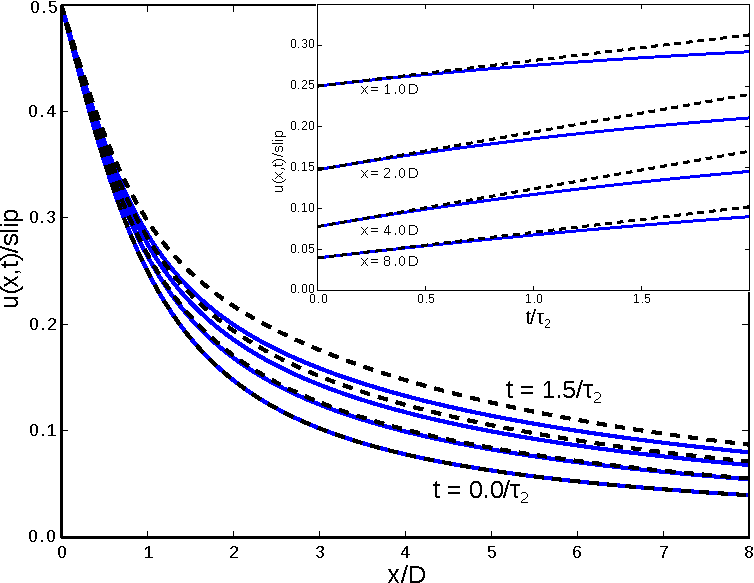
\includegraphics[width=0.8\textwidth]{FinalFigures/Figure1.pdf}
  \caption{Surface displacements predicted by
    eq. (\ref{TwoLayerViscous}) truncated after five terms (blue) and
    the approximation given by eq. (\ref{TwoLayerViscousApprox})
    (dotted black).  Displacements are shown at times 0, 5, 10, and 15
    years following an earthquake}
  \label{figure 1}
\end{figure}

\begin{figure}[h!]\label{figure2}
  \centering
  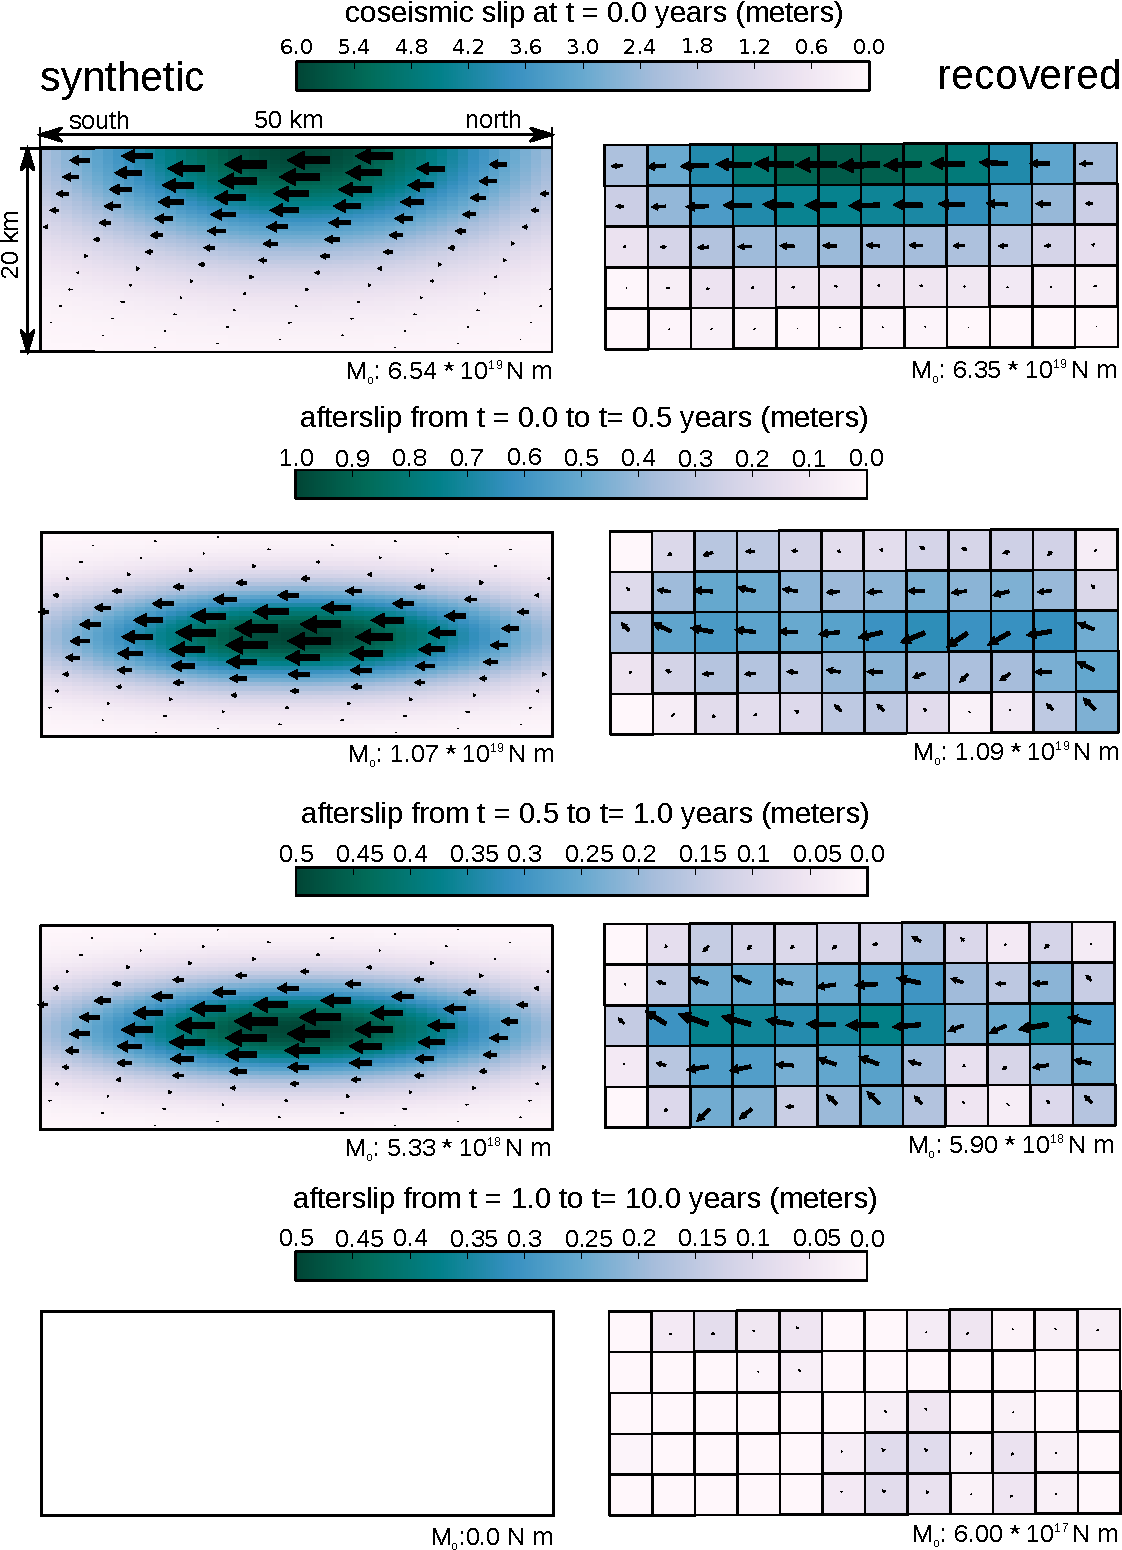
\includegraphics[width=0.9\textwidth]{FinalFigures/Figure2.pdf}
  \caption{Left: slip distribution imposed in the synthetic model.
    The panels from top to bottom represent coseismic slip at time =
    0.0, and afterslip over the period 0.0 to 0.5 years, 0.5 to 1.0
    years, and 1.0 to 10.0 years.  Colors indicate magnitude of slip
    and arrows indicate direction of slip.  Right: Slip recovered from
    inverting the synthetic surface deformation.}
  \label{figure 2}
\end{figure}

\begin{figure}[h!]\label{figure3}
  \centering
  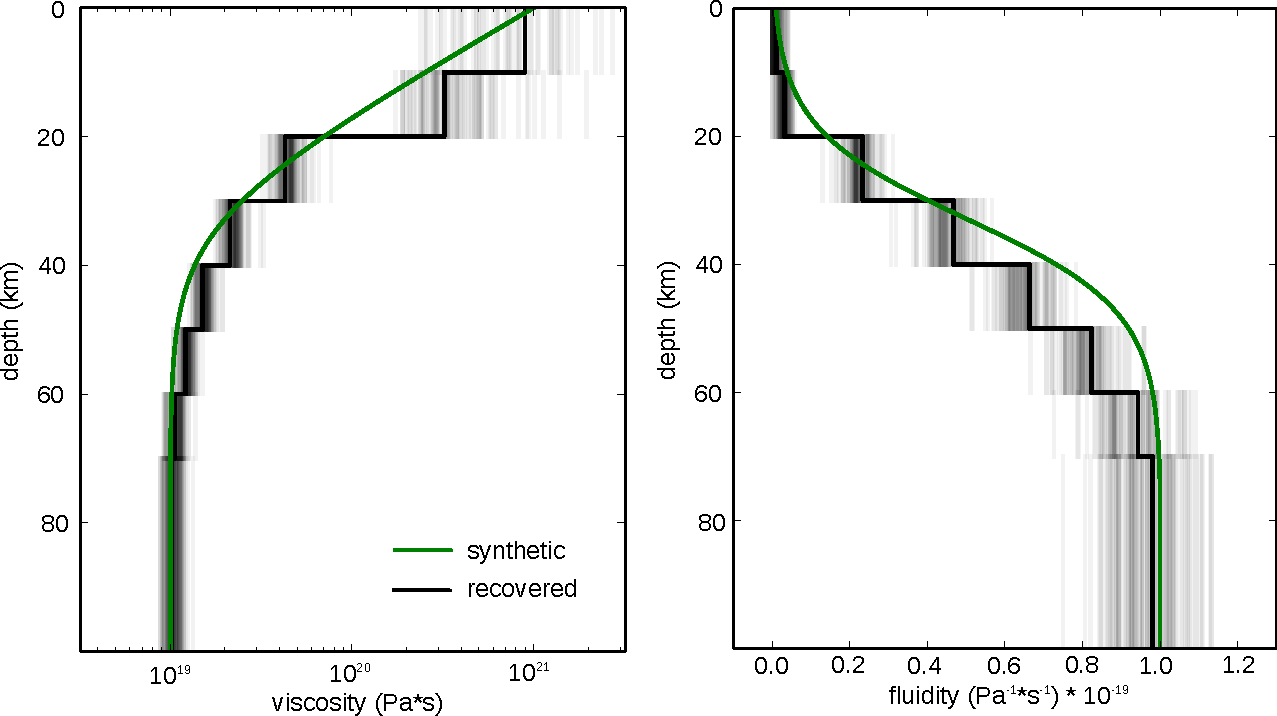
\includegraphics[width=0.9\textwidth]{FinalFigures/Figure3.pdf}
  \caption{Synthetic and recovered lithospheric viscosity strucutures.
    Blue line indicates viscosity structure imposed in the synthetic
    test. Black line indicates viscosity structure inferred from the
    synthetic surface displacement.  Semi-transparent lines are
    recovered models found through bootstrapping and indicate the
    degree of uncertainty on the inferred viscosity structure.  The
    left and right panels show the same information under
    different projections}
  \label{figure 3}
\end{figure}

\begin{figure}[h!]\label{figure4}
  \centering
  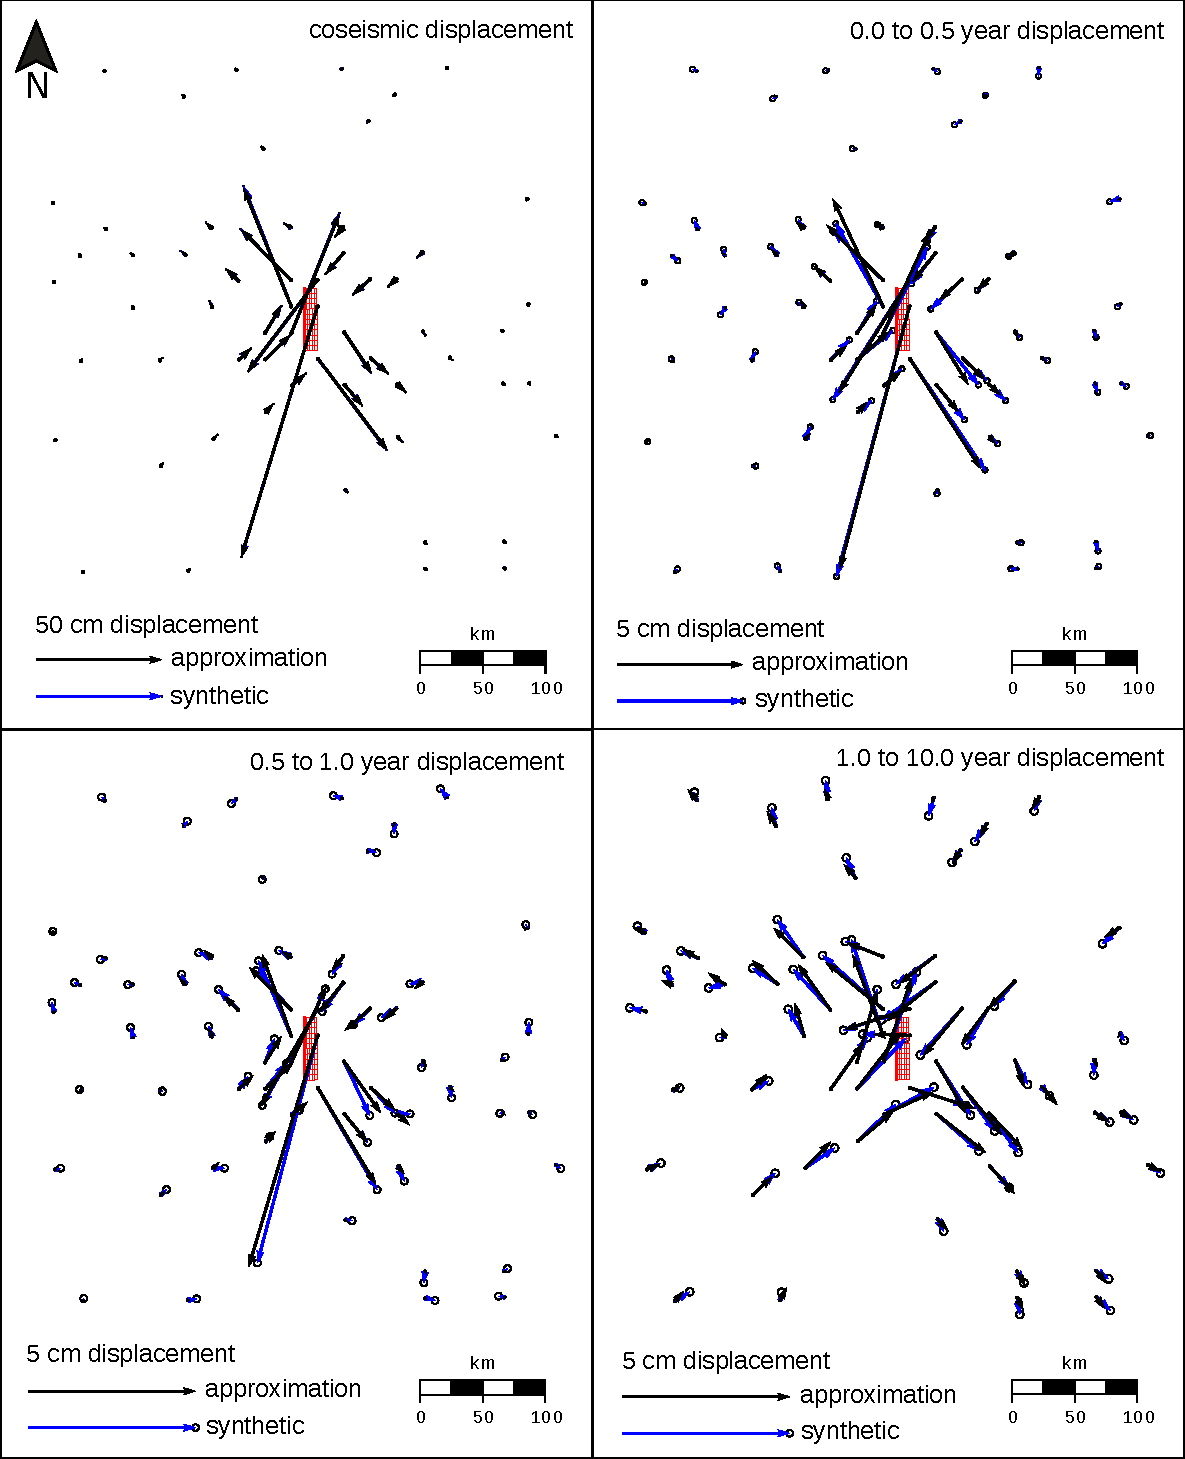
\includegraphics[width=0.9\textwidth]{FinalFigures/Figure4.pdf}
  \caption{Synthetic surface displacements (blue) and best fitting
    surface displacements (black).  Vertical displacements are used in
    the inversion but are not shown here.  The top left panel shows
    coseismic displacements and the remaining panals show the
    displacements over the indicated time intervals. Red dot indicates
    the position whos time series is shown in figure 5}
  \label{figure 4}
\end{figure}

\begin{figure}[h!]\label{figure5}
  \centering
  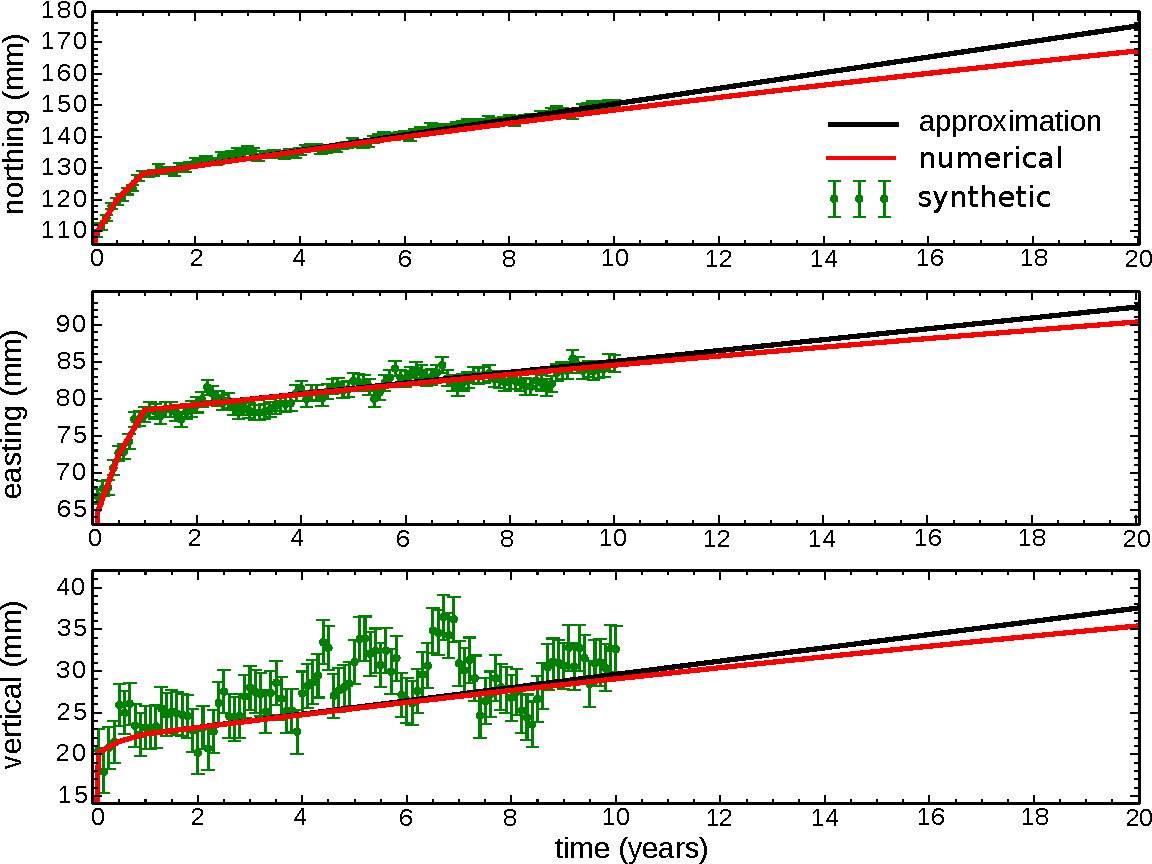
\includegraphics[width=0.9\textwidth]{FinalFigures/Figure5.pdf}
  \caption{Displacement time series for the position shown in figure 4
    (blue) and best fitting surface displacements using the
    approximation from eq. (\ref{Postseismic_Approximation}) (black).
    The red line indicates surface displacements computed using Pylith
    where the inferred slip distribution and viscosity structure are
    used as input.  The longevity of the approximation is
    indicated by when the black are red lines diverge}
  \label{figure 5}
\end{figure}

%\begin{figure}[h!]\label{figure6}
%  \centering
%  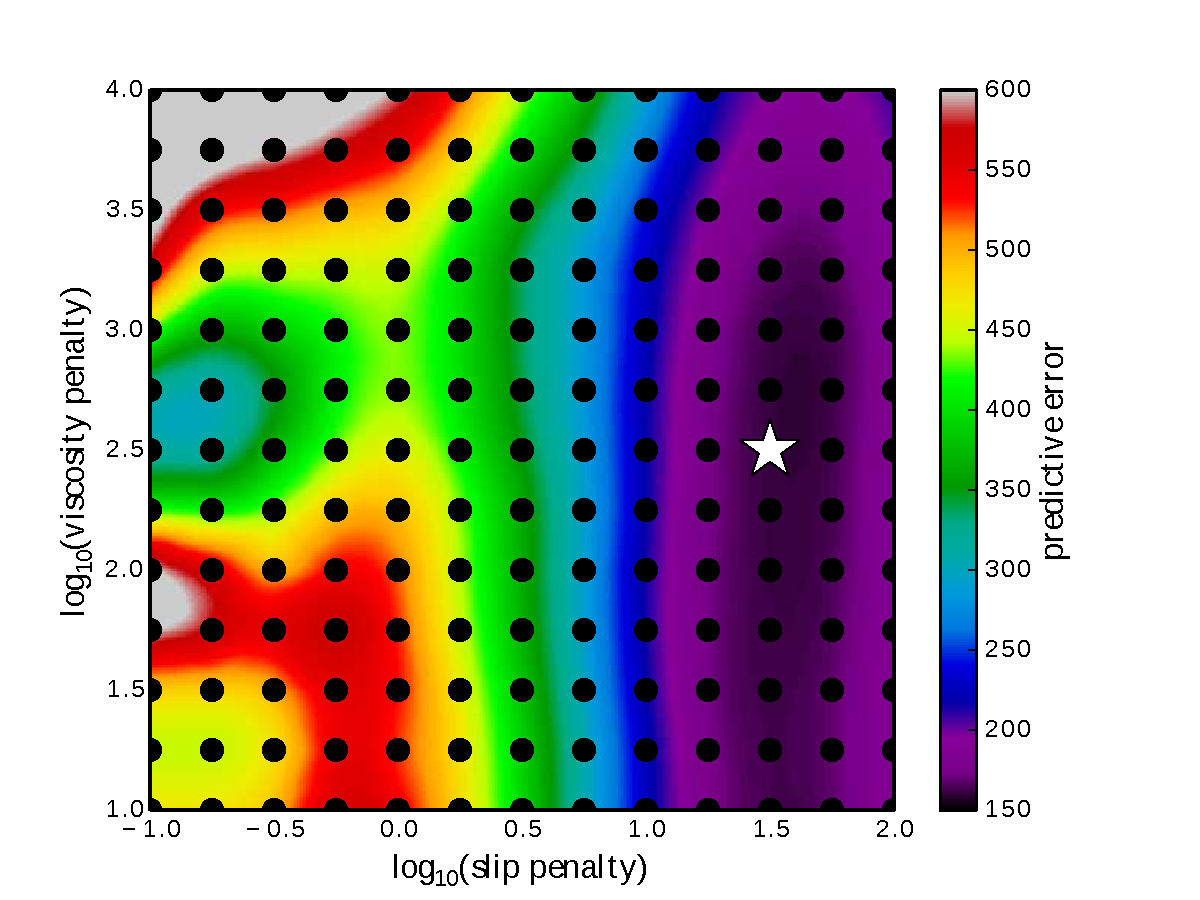
\includegraphics[width=0.9\textwidth]{FinalFigures/Figure6.pdf}
%  \caption{Predictive error for various pairs of slip and viscosity
%    penalty parameters.  Values are interpolated from the predictive
%    errors computed at each of the black dots.  The optimal pair of
%    penalty parameters produce the minimum predictive error and are
%    indicated by the star.}
%  \label{figure 6}
%\end{figure}

\begin{figure}[h!]\label{figure6}
  \centering
  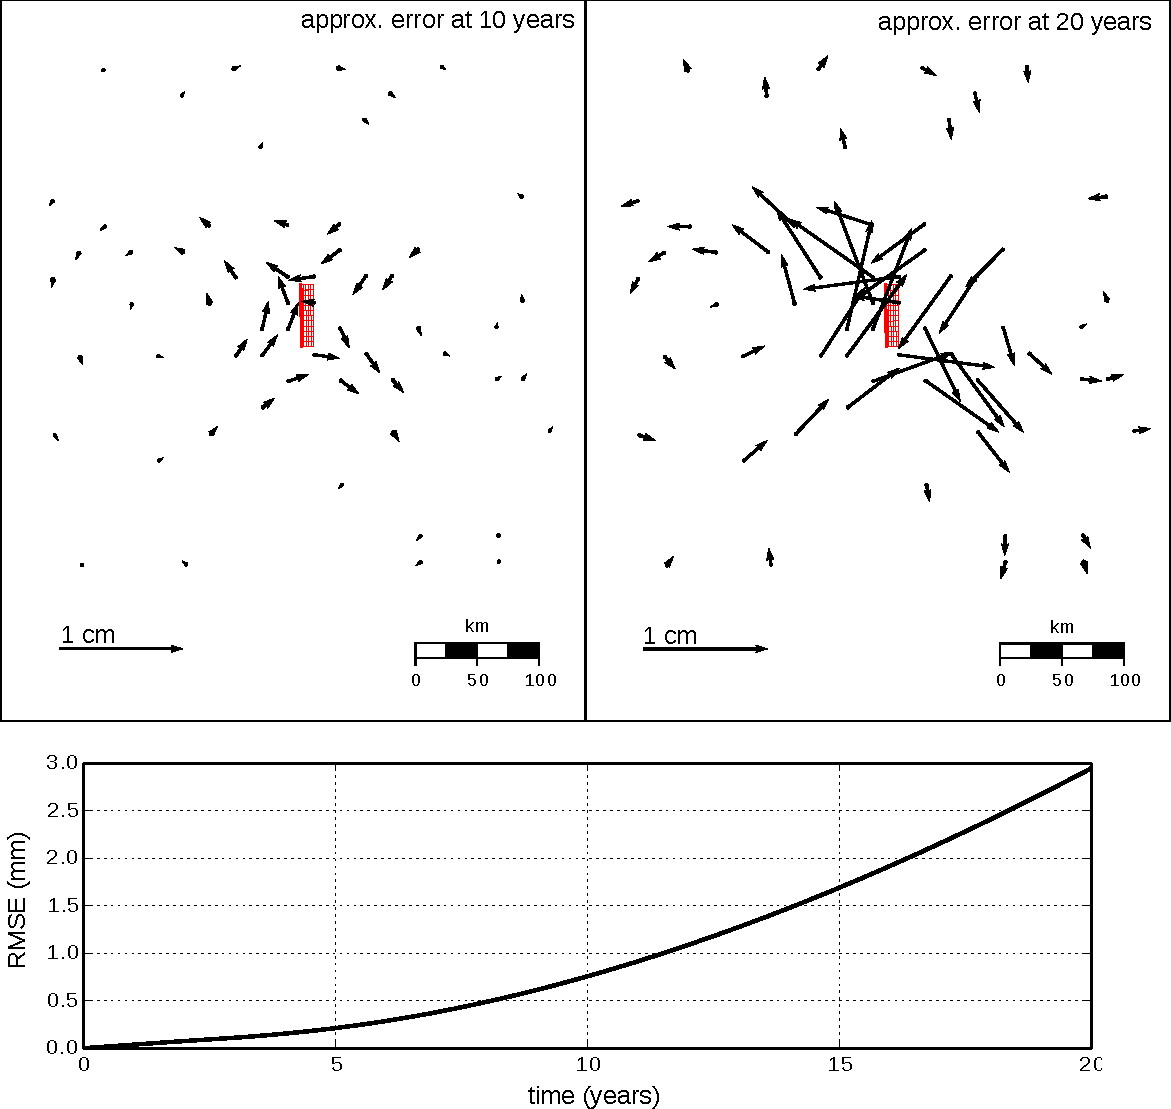
\includegraphics[width=0.9\textwidth]{FinalFigures/Figure7.pdf}
  \caption{Difference between the surface displacement approximation
    and the numerically computed surface displacements.  Top left
    panel shows the difference 10 years after the earthquake and the
    top right panel shows the difference at 20 years.  The bottom
    panel shows the root mean square of the approximation error over
    time.}
  \label{figure 6}
\end{figure}


\end{document}
